% Pregunta 3

\section*{Pregunta 3}
En la red de comunicaciones de 4 componentes conectados, la probabilidad de que funcione cada uno de los componentes es independiente de los demás, siendo la probabilidad de que funcione el componente 1 de 0.9, el componente 2 de 0.8, el componente 3 de 0.75 y el componente 4 de 0.85. La red funciona si entre A y B es posible encontrar un camino de componentes que funcione. Con los supuestos anteriores, calcular la probabilidad de que no haya comunicación entre A y B.

\begin{figure}[H]
	\centering
	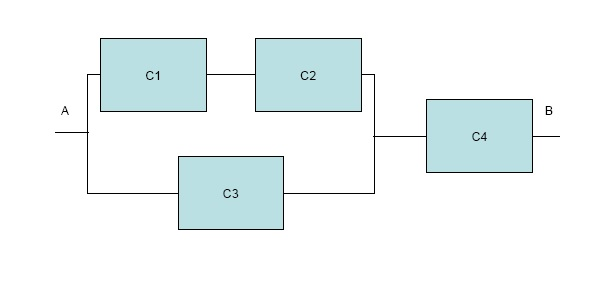
\includegraphics[scale=0.65]{img/ejercicio3.jpg}
\end{figure}

\textbf{R}: Definiremos el evento $F$ como el evento de que la red funcione, y por lo tanto la probabilidad de $F$ seria:
\begin{align*}
	\prob{F} 
	& = \prob{ \left( \left( C_1 \cap C_2 \right) \cup C_3 \right) \cap C_4 } \\
	& = \prob{ \left( C_1 \cap C_2 \right) \cup C_3 } \times \prob{C_4} \\
	& = \left( 1 - \prob{ \left( \overline{C_1} \cup \overline{C_2} \right) \cap \overline{C_3} } \right)  \times \prob{C_4} \\
	& = \left( 1 - \left( \prob{ \overline{C_1} \cup \overline{C_2} } \times \prob{\overline{C_3}} \right) \right)  \times \prob{C_4} \\
	& = \left( 1 - \left( \left( 1 - \prob{C_1 \cap C_2} \right) \times \prob{\overline{C_3}} \right) \right) \times \prob{C_4} \\
	& = \left( 1 - \left( \left( 1 - \left( \prob{C_1} \times \prob{C_2} \right)  \right) \times \prob{\overline{C_3}} \right) \right) \times \prob{C_4} \\
	& = \left( 1 - \left( \left( 1 - \left( 0.9 \times 0.8 \right)  \right) \times 0.25 \right) \right) \times 0.85 \\
	& = 0.7905
\end{align*}
Teniendo ña $\prob{F}$ podemos calcular la $\prob{\overline{F}}$, que seria la probabilidad de que la red no funcione, osea que no haya comunicación entre A y B.
\begin{align*}
	\prob{\overline{F}} = 1 - \prob{F} = 1 - 0.7905 = 0.2095
\end{align*}
Entonces la probabilidad de que no haya comunicación entre A y B es $20.95\%$.

